\documentclass[../DoAn.tex]{subfiles}
\begin{document}

\section{Hình học camera và phép chiếu phối cảnh}

Trong hệ camera lỗ kim, một điểm 3D $\mathbf{X}$ trong không gian được chiếu lên ảnh thông qua ma trận nội tại $K$ và ngoại tại $[R|t]$. Ở dạng thuần nhất:
\[
\mathbf{x} \sim K [R|t] \mathbf{X}.
\]
Trong các pipeline multi-view, việc ước lượng chính xác pose camera và mối quan hệ hình học giữa các ảnh là điều kiện tiên quyết để có thể khôi phục geometry ổn định.

\begin{figure}[H]
\centering
\resizebox{0.78\textwidth}{!}{%
\begin{tikzpicture}[
  cam/.style={draw=black!70, fill=gray!12, thick},
  plane/.style={draw=blue!60, fill=blue!8, thick},
  ray/.style={-{Latex[length=2.5mm]}, red!70!black, thick},
  guide/.style={dashed, gray!70},
  every node/.style={font=\small}
]
% camera 1
\draw[cam] (-4.8,0) -- (-4.1,0.45) -- (-4.1,-0.45) -- cycle;
\draw[plane] (-3.25,-0.95) rectangle (-3.0,0.95);
\node at (-4.55,-0.8) {$C_1$};
\node[blue!60!black] at (-3.12,1.2) {mặt phẳng ảnh 1};
% camera 2
\draw[cam] (4.8,0) -- (4.1,0.45) -- (4.1,-0.45) -- cycle;
\draw[plane] (3.0,-0.95) rectangle (3.25,0.95);
\node at (4.55,-0.8) {$C_2$};
\node[blue!60!black] at (3.12,1.2) {mặt phẳng ảnh 2};
% world point
\filldraw[red!80!black] (0,1.1) circle (2.2pt);
\node[above] at (0,1.1) {điểm 3D $\mathbf{X}$};
% rays
\draw[ray] (-4.35,0) -- (0,1.1);
\draw[ray] (4.35,0) -- (0,1.1);
% image projections
\filldraw[red!80!black] (-3.12,0.3) circle (2pt);
\filldraw[red!80!black] (3.12,0.3) circle (2pt);
\node[left] at (-3.18,0.3) {$\mathbf{x}_1$};
\node[right] at (3.18,0.3) {$\mathbf{x}_2$};
\draw[guide] (0,1.1) -- (-3.12,0.3);
\draw[guide] (0,1.1) -- (3.12,0.3);
\end{tikzpicture}
}
\caption{Minh họa hình học camera đa góc nhìn trong tái tạo 3D từ ảnh UAV. Hai camera quan sát cùng một điểm 3D từ các pose khác nhau; từ các phép chiếu tương ứng, hệ thống có thể suy ra pose, depth và cấu trúc scene.}
\label{fig:multi-view-geometry}
\end{figure}

\section{Depth map, point cloud và pointmap}

Depth map biểu diễn khoảng cách từ camera tới bề mặt scene tại từng pixel. Point cloud là tập các điểm 3D trong hệ tọa độ thế giới hoặc hệ camera. Pointmap trong các mô hình như DUSt3R là một cách dự báo trực tiếp ánh xạ từ pixel sang tọa độ 3D, giúp đơn giản hóa nhiều bước ràng buộc projective cổ điển.

\begin{figure}[H]
\centering
\begin{minipage}[t]{0.31\textwidth}
  \centering
  
\includegraphics[width=\linewidth]{figures/dronescapes_risk_depth.pdf}

  \scriptsize (a) Depth map
\end{minipage}
\hfill
\begin{minipage}[t]{0.31\textwidth}
  \centering
  
\includegraphics[width=\linewidth]{figures/odmdata_openmvs_pointcloud.pdf}

  \scriptsize (b) Point cloud
\end{minipage}
\hfill
\begin{minipage}[t]{0.31\textwidth}
  \centering
  \begin{tikzpicture}[scale=0.8, every node/.style={font=\scriptsize}]
    \draw[fill=gray!12, draw=black!70] (-1.3,-1.0) rectangle (0.2,1.0);
    \draw[step=0.3, gray!55] (-1.3,-1.0) grid (0.2,1.0);
    \node at (-0.55,1.25) {pixel grid};
    \foreach \x/\y/\tx/\ty in {-1.05/0.65/1.1/1.0,-0.75/0.05/1.45/0.4,-0.45/-0.55/0.95/-0.65,-1.15/-0.2/1.65/-0.1}{
      \fill[red!70!black] (\x,\y) circle (1.8pt);
      \fill[blue!65] (\tx,\ty) circle (2pt);
      \draw[->, thick, orange!80!black] (\x,\y) -- (\tx,\ty);
    }
    \draw[thick] (1.0,-0.9) -- (2.0,-0.5) -- (1.6,0.9);
    \draw[thick] (1.0,-0.9) -- (1.25,-0.15) -- (1.6,0.9);
    \draw[thick] (2.0,-0.5) -- (1.25,-0.15);
    \node at (1.35,1.25) {tọa độ 3D};
    \node[align=center] at (0.4,-1.35) {Pointmap: mỗi pixel\\được ánh xạ sang một điểm 3D};
  \end{tikzpicture}

  \scriptsize (c) Pointmap
\end{minipage}
\caption{Ba kiểu biểu diễn hình học xuất hiện xuyên suốt đồ án. Depth map thuận tiện cho đánh giá theo pixel; point cloud phù hợp quan sát cấu trúc scene; pointmap giúp mô hình học sâu dự báo trực tiếp hình học 3D từ miền ảnh.}
\label{fig:depth-pointcloud-pointmap}
\end{figure}

\section{Các yếu tố làm khó tái tạo UAV}

Với ảnh UAV, các khó khăn chính thường đến từ:
\begin{enumerate}[leftmargin=1.5em]
  \item texture yếu hoặc lặp lại, khiến matching kém ổn định;
  \item overlap không đều giữa các ảnh;
  \item góc nhìn bất lợi, đặc biệt với các cấu trúc hẹp hoặc che khuất;
  \item thay đổi cao độ, ánh sáng, hoặc cảnh quá rộng làm tăng chi phí tính toán.
\end{enumerate}

Những yếu tố này chính là nền tảng để xây dựng một thước đo \textit{reconstruction risk}.

\begin{figure}[H]
\centering
\begin{minipage}[t]{0.47\textwidth}
\centering
\resizebox{0.95\linewidth}{!}{%
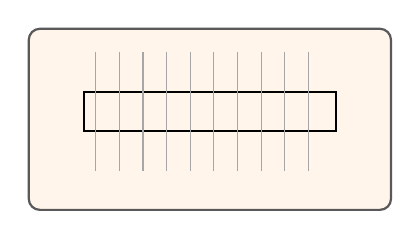
\begin{tikzpicture}[every node/.style={font=\scriptsize}]
\draw[rounded corners, draw=black!65, thick, fill=orange!8] (-2.3,-1.15) rectangle (2.3,1.15);
\draw[thick] (-1.6,-0.15) rectangle (1.6,0.35);
\foreach \x in {-1.45,-1.15,-0.85,-0.55,-0.25,0.05,0.35,0.65,0.95,1.25}{
  \draw[gray!70] (\x,-0.65) -- (\x,0.85);
}
\end{tikzpicture}
}

{\scriptsize \textbf{(a) Texture yếu hoặc lặp lại.} Matching dễ mơ hồ ở mái nhà, đường, đồng cỏ hoặc các mặt phẳng lớn.}
\end{minipage}
\hfill
\begin{minipage}[t]{0.47\textwidth}
\centering
\resizebox{0.95\linewidth}{!}{%
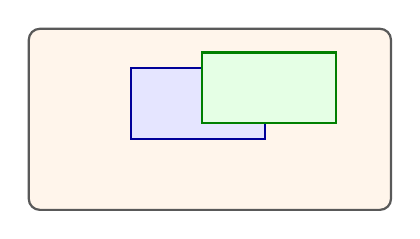
\begin{tikzpicture}[every node/.style={font=\scriptsize}]
\draw[rounded corners, draw=black!65, thick, fill=orange!8] (-2.3,-1.15) rectangle (2.3,1.15);
\draw[fill=blue!10, draw=blue!60!black, thick] (-1.0,-0.25) rectangle (0.7,0.65);
\draw[fill=green!10, draw=green!50!black, thick] (-0.1,-0.05) rectangle (1.6,0.85);
\end{tikzpicture}
}

{\scriptsize \textbf{(b) Overlap không đều.} Các cặp ảnh hỗ trợ hình học không phân bố đồng đều trên toàn block bay.}
\end{minipage}

\vspace{0.7em}

\begin{minipage}[t]{0.47\textwidth}
\centering
\resizebox{0.95\linewidth}{!}{%
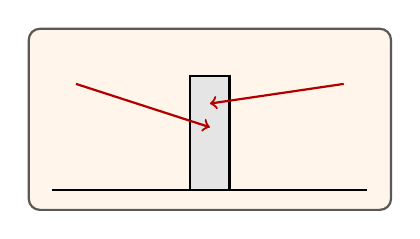
\begin{tikzpicture}[every node/.style={font=\scriptsize}]
\draw[rounded corners, draw=black!65, thick, fill=orange!8] (-2.3,-1.15) rectangle (2.3,1.15);
\draw[thick] (-2.0,-0.9) -- (2.0,-0.9);
\draw[thick, fill=gray!20] (-0.25,-0.9) rectangle (0.25,0.55);
\draw[->, thick, red!70!black] (-1.7,0.45) -- (0.0,-0.1);
\draw[->, thick, red!70!black] (1.7,0.45) -- (0.0,0.2);
\end{tikzpicture}
}

{\scriptsize \textbf{(c) Góc nhìn bất lợi và che khuất.} Vật thể mảnh, góc xiên và vùng bị che làm depth suy giảm ổn định.}
\end{minipage}
\hfill
\begin{minipage}[t]{0.47\textwidth}
\centering
\resizebox{0.95\linewidth}{!}{%
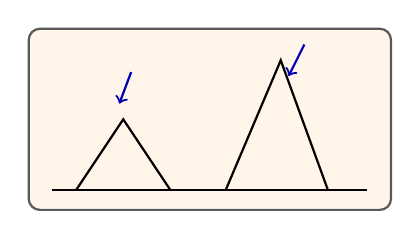
\begin{tikzpicture}[every node/.style={font=\scriptsize}]
\draw[rounded corners, draw=black!65, thick, fill=orange!8] (-2.3,-1.15) rectangle (2.3,1.15);
\draw[thick] (-2.0,-0.9) -- (2.0,-0.9);
\draw[thick] (-1.7,-0.9) -- (-1.1,0.0) -- (-0.5,-0.9);
\draw[thick] (0.2,-0.9) -- (0.9,0.75) -- (1.5,-0.9);
\draw[->, thick, blue!70!black] (-1.0,0.6) -- (-1.15,0.2);
\draw[->, thick, blue!70!black] (1.2,0.95) -- (1.0,0.55);
\end{tikzpicture}
}

{\scriptsize \textbf{(d) Biến thiên cao độ và tỉ lệ.} Đồi dốc hoặc đô thị dày đặc làm thay đổi scale, depth range và phân bố lỗi.}
\end{minipage}
\caption{Bốn tình huống điển hình khiến tái tạo UAV khó ổn định. Đây cũng là các tín hiệu trực giác được chuyển hóa thành những thành phần của risk score trong đồ án.}
\label{fig:uav-difficulty-factors}
\end{figure}

\section{Khái niệm risk score trong đề tài}

Đề tài không học trực tiếp uncertainty bằng một mạng riêng, mà dùng một thước đo heuristic ở mức frame. Mục tiêu của risk score không phải dự báo sai số tuyệt đối, mà trả lời câu hỏi thực dụng hơn: frame nào đáng được refine trước nếu chỉ có một ngân sách hữu hạn?

\begin{figure}[H]
\centering
\begin{tikzpicture}[
  every node/.style={font=\small},
  sel/.style={fill=red!70!black},
  base/.style={fill=blue!55}
]
\draw[->, thick] (0,0) -- (9.2,0) node[right] {frame};
\draw[->, thick] (0,0) -- (0,4.8) node[above] {risk};
\foreach \x/\h/\label in {0.7/1.1/F1,1.7/2.7/F2,2.7/1.8/F3,3.7/4.0/F4,4.7/1.5/F5,5.7/3.6/F6,6.7/0.9/F7,7.7/3.1/F8}{
  \ifdim \h pt>3.0pt
    \fill[sel] (\x,0) rectangle +(0.65,\h);
  \else
    \fill[base] (\x,0) rectangle +(0.65,\h);
  \fi
  \node[below] at (\x+0.325,0) {\label};
}
\draw[dashed, gray!70] (0,3.0) -- (8.7,3.0);
\node[gray!70, anchor=west] at (8.75,3.0) {ngưỡng chọn top-$K$};
\node[align=center] at (4.4,4.35) {\textbf{Các frame rủi ro cao}\\được ưu tiên refine};
\end{tikzpicture}
\caption{Ví dụ trực quan của cơ chế risk-guided selection trong đồ án. Những frame có điểm rủi ro cao hơn được ưu tiên đưa vào nhánh refine, thay vì chạy refinement đồng đều trên toàn bộ chuỗi ảnh.}
\label{fig:risk-selection-theory}
\end{figure}

\end{document}
